\begin{center}
    \textbf{Geração 20}
\end{center}

\begin{figure}[h]
    \centering
    \label{fig:geracao01}
    
    \begin{tabular}{rl}
        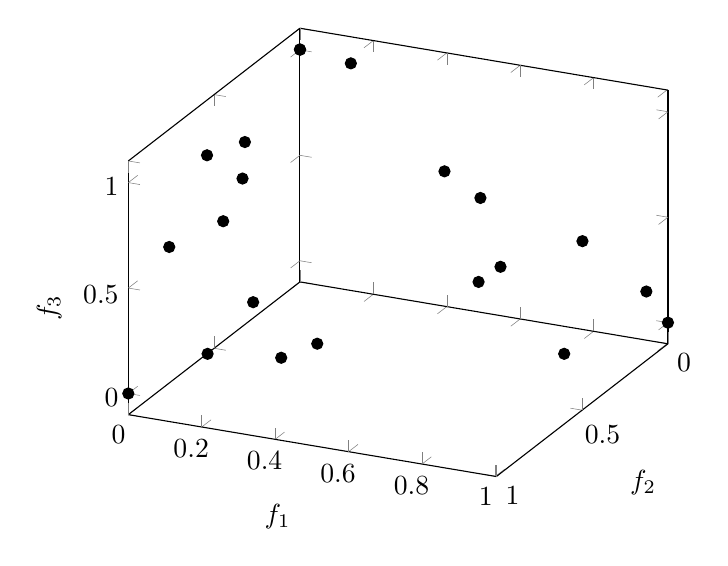
\begin{tikzpicture}[scale=1.0]
        	\begin{axis}[xlabel=$f_2$, ylabel=$f_1$, zlabel=$f_3$, view/h=115]
        		
    			\addplot3[only marks] coordinates {
            		(1.000002, 0.000000, 0.000000) (0.000000, 1.002468, 0.000000) (0.541310, 0.000000, 0.840826) (0.000000, 0.000433, 1.000496) (0.000000, 0.000000, 1.002320) (0.722187, 0.128600, 0.679644) (0.811987, 0.023568, 0.583289) (0.197183, 0.861776, 0.469365) (0.406695, 0.909961, 0.081084) (0.957202, 0.195942, 0.218489) (0.903834, 0.371536, 0.217686) (0.863512, 0.276258, 0.427933) (0.315326, 0.541161, 0.780902) (0.472791, 0.071105, 0.881298) (0.016394, 0.146355, 0.989118) (0.450001, 0.756722, 0.476101) (0.591568, 0.120165, 0.797279) (0.326372, 0.644212, 0.691721) (0.077636, 0.979919, 0.189924) (0.853004, 0.445917, 0.274074) (0.521535, 0.730392, 0.441699) 


        		};
        	\end{axis}
	    \end{tikzpicture}
	    &
	    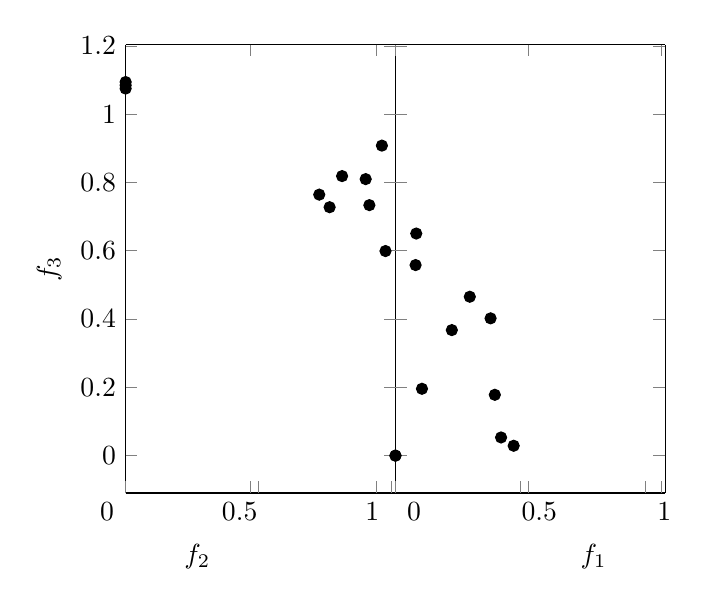
\begin{tikzpicture}[scale=1.0]
        	\begin{axis}[xlabel=$f_2$, ylabel=$f_1$, zlabel=$f_3$, view={45}{0}]
        		\addplot3[only marks] coordinates {
            		(1.016495,0.000000,0.000000)(0.000000,1.078561,0.000000)(0.000000,0.000000,1.074789)(0.000000,0.000000,1.084236)(0.000000,0.000000,1.093925)(0.635397,0.350182,0.907756)(0.182853,0.990524,0.195721)(0.520405,0.609485,0.650315)(0.962224,0.479792,0.053201)(0.310600,0.644734,0.733455)(0.032921,0.780486,0.727344)(0.131020,0.726226,0.818520)(0.693930,0.037634,0.764224)(0.924342,0.394941,0.465204)(0.756570,0.748373,0.028904)(0.919474,0.500193,0.178071)(0.412651,0.866068,0.367581)(0.238939,0.905559,0.557961)(0.691780,0.724817,0.402005)(0.216007,0.809554,0.599020)(0.555754,0.369831,0.809650)
        		};
        	\end{axis}
	    \end{tikzpicture}
	\end{tabular}
    
\end{figure}

